\documentclass{standalone}
\usepackage{amsmath}
\usepackage{amsfonts}
\usepackage{tikz}
\usetikzlibrary{arrows,shapes,positioning,shadows,trees}

\begin{document}
\begin{tikzpicture}
    \node (a) at (0,0) {
        \begin{tikzpicture}
            \filldraw[fill=gray!30, draw=black] (0,1.732) circle (2);
            \filldraw[fill=white, draw=black] (0,0) circle (1);
            \draw[->] (-2,0) -- (2,0);
            \draw[->] (0,-2) -- (0,4);
            \draw (0,0) circle (1);
            \draw (0,1.732) circle (2);
            \node[fill,circle,inner sep=1pt,label=above right:$\sqrt{3}i$] at (0,1.732) {};
            \node[fill,circle,inner sep=1pt,label=below left:$-1$] at (-1,0) {};
            \node[fill,circle,inner sep=1pt] at (0,0) {};
            \node[fill,circle,inner sep=1pt] at (1,0) {};
        \end{tikzpicture}
    };

    \node(b) at (6,0) {
        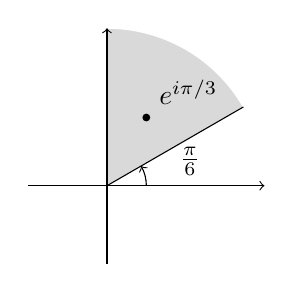
\begin{tikzpicture}
            \filldraw[fill=gray!30, draw=white!0] (0,0) -- (1.732,1) arc (30:90:2) -- (0,0);
            \draw[->] (-1,0) -- (2,0);
            \draw[->] (0,-1) -- (0,2);
            \draw[-] (0,0) -- (1.732, 1);
            \draw[->] (0.5,0) arc (0:30:0.5);
            \node[above right] at (0.8,0) {$\frac{\pi}{6}$};
            \node[fill,circle,inner sep=1pt,label=above right:$e^{i\pi/3}$] at (1 / 2,1.732 / 2) {};
        \end{tikzpicture}
    };

    \node (c) at (12,0) {
        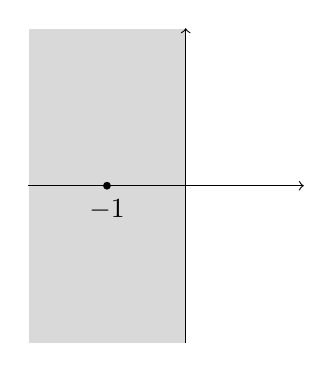
\begin{tikzpicture}
            \filldraw[fill=gray!30, draw=white!0] (-2,2) -- (-2,-2) -- (0,-2) -- (0,2) -- (-2,2);
            \draw[->] (-2,0) -- (1.5,0);
            \draw[->] (0,-2) -- (0,2);
            \node[fill,circle,inner sep=1pt,label=below:$-1$] at (-1,0) {};
        \end{tikzpicture}
    };

    \node (d) at (18,0) {
        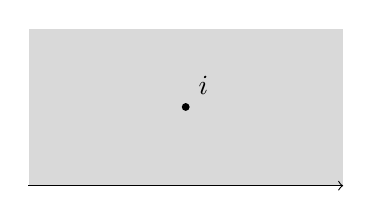
\begin{tikzpicture}
            \filldraw[fill=gray!30, draw=white!0] (-2,2) -- (-2,0) -- (2,0) -- (2,2) -- (-2,2);
            \draw[->] (-2,0) -- (2,0);
            \node[fill,circle,inner sep=1pt,label=above right:$i$] at (0,1) {};
        \end{tikzpicture}
    };

    \node (e) at (24,0) {
        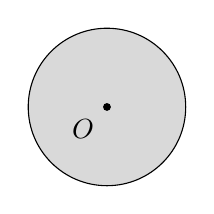
\begin{tikzpicture}
            \filldraw[fill=gray!30] (0,0) circle (1);
            \node[fill,circle,inner sep=1pt,label=below left:$O$] at (0,0) {};
        \end{tikzpicture}
    };

    \draw[->,thick] (a) -- (b) node[midway,above] {$f(z) = \dfrac{z+1}{z-1}$};
    \draw[->,thick] (b) -- (c) node[midway,above] {$f(z) = z^3$};
    \draw[->,thick] (c) -- (d) node[midway,above] {$f(z) = -iz$};
    \draw[->,thick] (d) -- (e) node[midway,above] {$f(z) = e^{i\theta}\cdot\dfrac{z-i}{z+i}$};
\end{tikzpicture}

\end{document}